%%%%%%%%%%%%%%%%%%%%%%%%%%%%%%%%%%%%%%%%%%%%%%%%%%%%%%%%%%%%%%%%%%%%%%%%%%%%%%%
%%                                                    DATA SIMULATION SELECTION
%%%%%%%%%%%%%%%%%%%%%%%%%%%%%%%%%%%%%%%%%%%%%%%%%%%%%%%%%%%%%%%%%%%%%%%%%%%%%%%
%%                                    about the samples, MC Generation and cuts 



%______________________________________________________________________________
%                                                Daten Simulation und Selektion 
\chapter{Daten, Simulation \& Selektion}

\begin{quote}
    The abstract come last
\end{quote}



%______________________________________________________________________________
%                                                                         Daten 
\section{Daten}
\label{data_sim_selection:data}

% + Daten von 2012
% + Parameter: Energie, Bunchespacing, Perioden
% + Energie-Kalibration

Die Daten, die dieser Arbeit zugrunde liegen, wurden vom ATLAS-Detektor im Jahr
2012 bei erstmalig $8 \TeV$ Schwerpunktsenergie aufgenommen. Der \ac{LHC} wird
mit Paketen von Protonen, sogenannte Bunches (vom engl. Bunch: Bündel) gefüllt,
die für einige Stunden im Beschleuniger zirkulieren\footnote{weitere Details:
siehe Kapitel \ref{}}.
Eine solche Füllung steht für identische Einstellungen des Beschleunigers bzw.
Detektors und wird in ATLAS mit einer fortlaufenden Nummer identifiziert.
Die Füllungs-Nummern größerer Perioden konstanter Bedingungen, wie das zu der
Zeit implementierte Trigger-Menü oder globale \ac{LHC} Parameter, werden dann
mit einem Buchstaben zusammengefasst (Periode A, B, ...).

Der vorliegende Datensatz wurde in der Zeit zwischen dem 04. April 2012 und dem
16. Dezember 2012 aufgenommen und umfasst 10 Perioden, die einer integrierten
Gesamtluminosität von $20,3 \fb^{-1}$ entsprechen\footnote{nach Anwenung der
\ac{GRL} (siehe Kapitel \ref{})} (siehe Abbildung \ref{fig:lumi}). Der
Beschleuniger wurde hierbei in einer Konfiguration betrieben, die einen
zeitlichen Abstand zwischen den Teilchen-Paketen von $50\:\nano\second$
gewährleistet, woraus eine instantane Luminosität\footnote{Erläuterungen zur
Messung der Luminosität in ATLAS finden sich in Kapitel \ref{}} von bis zu
$7,73 \cdot 10^{-33} \centi\meter^{-2}\second^{-1}$ resultiert.

Eine hohe instantane Luminosität verspricht eine große Rate interessanter
Ereignisse, jedoch bedingt sie auch viele unerwünschte Neben-Ereignisse,
vorwiegend aus inelastischen Streuprozessen, die einen signifikanten Einfluss
auf die Messung nehmen können. Dieser Effekt wird als \textit{Pile-Up}
bezeichnet und ist in Abbildung \ref{fig:pileup} illustriert.

\begin{figure}
    \begin{minipage}[b]{0.48\textwidth}
        \centering
        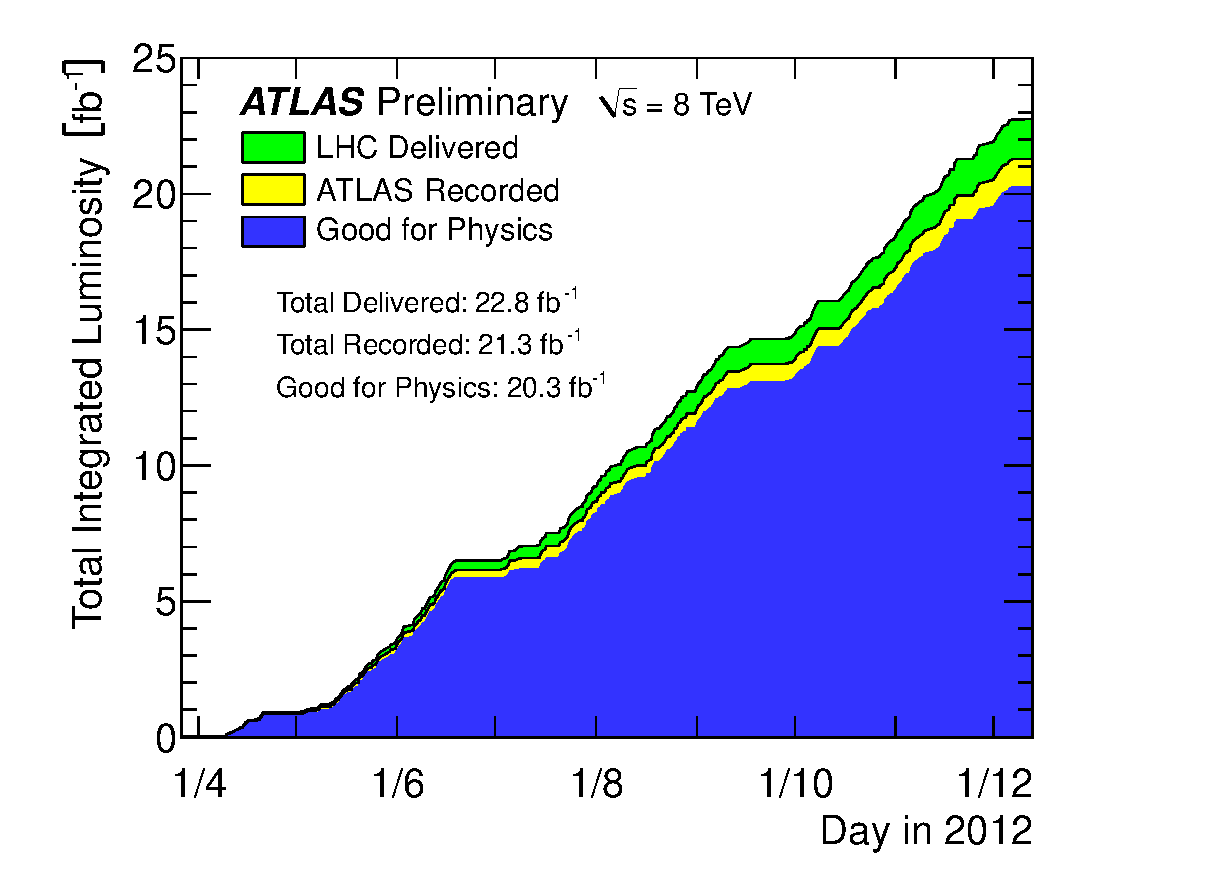
\includegraphics[width=1.\textwidth]{plots/lumi}
        \captionsetup{format=plain}
        \caption{Verfügbare, aufgezeichnete und validierte integrierte
            Luminosität aufgetragen gegen die Zeit innerhalb der Messkampange}
        \label{fig:lumi}
    \end{minipage}
    \hfill
    \begin{minipage}[b]{0.48\textwidth}
        \centering
        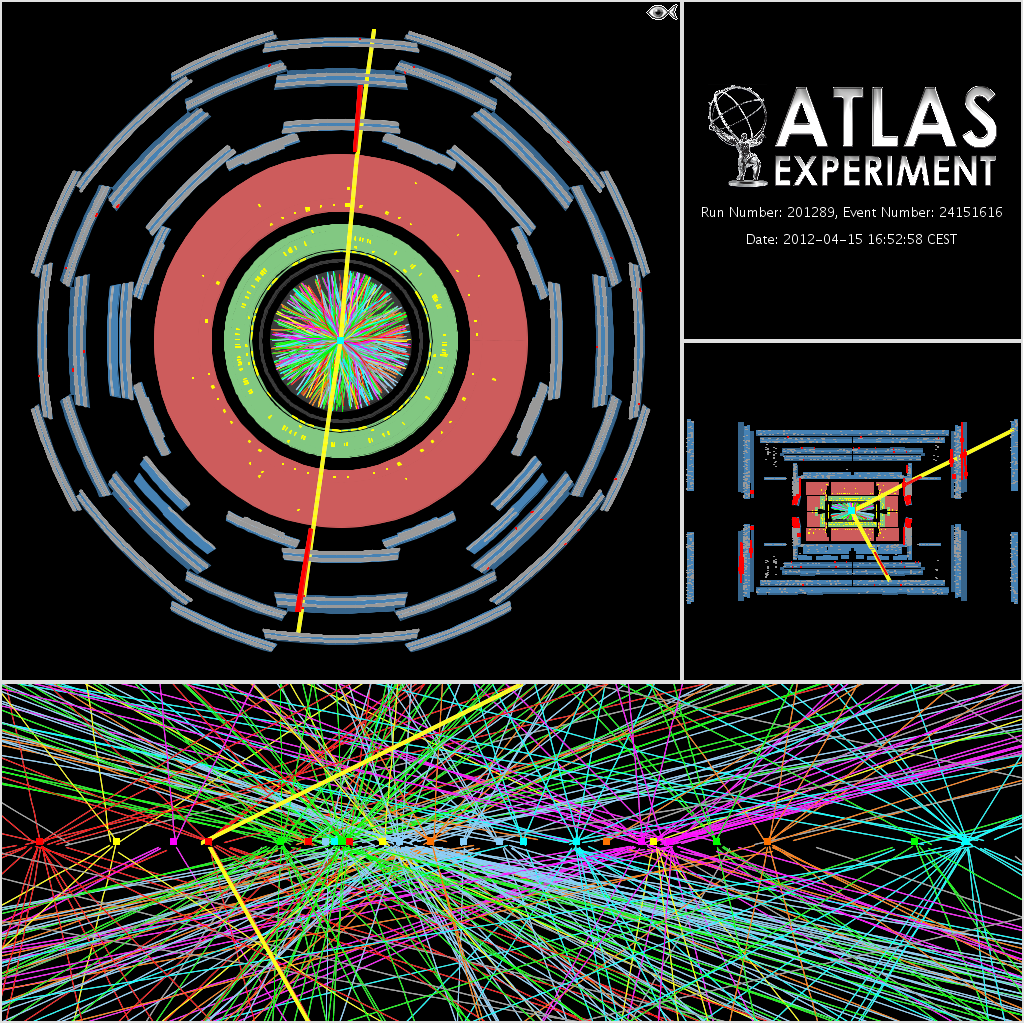
\includegraphics[width=1.\textwidth]{img/pileup}
        \captionsetup{format=plain}
        \caption{Ereignisse mit $Z \rightarrow \mu\mu$ Kandidat und hohem
            Pile-Up. 25 rekonstruierte Vertizes.}
        \label{fig:pileup}
    \end{minipage}
\end{figure}

Das in dieser Arbeit verwendete Speicherformat für Daten basiert auf den in
Abschnitt \ref{} beschriebenen D3PD Tupeln in SMWZ Konfiguration. Für die
Verwendung innerhalb der Arbeitsgruppe in Mainz wurden diese Tupel zum Zwecke
der Speicherplatz-Ersparnis auf Ereignisse beschnitten, die mindestens zwei
Elektronkandidaten mit je $23 \GeV$ bzw. $14 \GeV$ aufweisen.

Die Energie der Elektronkandidaten in diesen Tupeln beruht auf der Information
aus den Rekonstruktionsalgorithmen und bedarf noch der Kalibration. Für
Elektronen im Zentral-Bereich werden dazu Kalibrations-Faktoren benutzt, die
von der zuständigen ATLAS Arbeitsgruppe für die Kalibration des
elektromagnetischen Kalorimeters (\textit{Electron Gamma Working Group}, kurz:
egamma) bereitsgestellt werden. Für Elektronen im Vorwärts-Bereich wurden noch
keine Kalibrations-Faktoren bereitgestellt, weshalb diese in Kapitel
\ref{energy_calibration} dieser Arbeit selbst bestimmt werden.


%______________________________________________________________________________
%                                                                    Simulation
\section{Simulation}
\label{data_sim_selection:simulation}

% + Motivation für Simulation (Theorie-Vorhersage)
% + Mehrschrittiges Prinzip
% + Eventgeneration (Matrixelemente, Fragmentation,...)
% + Detektorsimulation (+ Ausgabeformat)
% + Nötige Korrekturen (Pileup, Effizienzen, Smearing, kFaktors)
% + Übersicht und kurze(!) Statements zu Samples
% + LumiScaling

Die Simulation von Ereignissen und des Detektors ist ein wichtiger Bestandteil
von Analysen in der Hochernergiephysik. Sie repräsentiert einerseits das
beste Wissen über die betrachteten Prozesse und die genaue Kenntnis des
Detektors, andererseits lassen sich mit Simulationen die Erweiterungen durch
neue theoretische Modelle untersuchen und deren Einfluss auf bereits bekannte
Prozesse vorhersagen. Zentraler Gegenstand der Betrachtung ist hierbei stets
der Vergleich zwischen Simulation und realen Daten.



\subsection{Erzeugung simulierter Datensätze}
\label{event_generation}
Die Erstellung einer Simulation, im folgenden meist nur noch als
\textit{Monte-Carlo} bezeichnet, geschieht für gewöhnlich in mehreren
Schritten. Eine grobe Unterteilung ist die Unterscheidung zwischen der
Simulation des eigentlichen physikalischen Prozesses, wie beispielsweise die
Annihilation eines Quarks und eines Antiquarks zu einem Z-Boson und dessen
nachfolgenden Zerfall in ein Leptonpaar, und die Simulation der
Detektorantwort, also der Beschreibung aller physikalischer Subprozesse, die
von den Produkt-Teilchen im Detektor induziert werden (Detektor-Antwort).

Im ersten Schritt, der Ereignis-Simulation, kommen so genannte
\textit{Monte-Carlo Generatoren} zum Einsatz. Dies sind meist von theoretischen
Physikern implementierte Software Pakete, die, hochkonfigurierbar, mittels
Zufallszahlen die gewünschten Prozesse, samt der kinematischen Parameter der
eingehenden und ausgehenden Teilchen als Ereignisse simulieren. Dies geschieht
auf der Basis von Matrixelementen und der Beschreibung des Phasenraumes. Die
voran gestellte Berechnung der Matrixelemente findet meist in führender (LO)
oder nächst-führender (NLO) Ordnung statt. Betrachtungen höherer Ordnungen
werden aufgrund der übermäßigen Komplexität in der Regel durch Umgewichtungen
von Simulationen niedrigerer Ordnung realisiert\footnote{siehe auch Abschnitt
\ref{mc_corrections}}. Neben dem harten Streuprozess inklusive aller
beteiligten Partonen werden anschließend weitere Effekte wie beispielsweise
Hadronisierung oder Bremsstrahlung berücksichtigt. Alle bis zu diesem Punkt
gewonnenen Werte bezeichnet man als \textit{Generator-Level}.

Die kinematische Information der Produkt-Teilchen auf Generator-Level wird nun
der Detektor-Simulation übergeben, welche die Wechselwirkung mit
Detektormaterial und die elektronische Antwort des Detektors beschreibt, sodass
an deren Ende ein mit realen Signalen vergleichbarer Datensatz entsteht. Diese
Aufgabe übernimmt in ATLAS das \textsc{GEANT4}-Paket\footnote{\textsc{GEANT4}:
Softwarepaket zur Simulation von Teilchen in Materie
(\cite{Agostinelli:2002hh})}, mithilfe dessen eine sehr detailgetreue virtuelle
Beschreibung des Detektors erstellt wurde.



\subsection{Korrekturen}
\label{mc_corrections}
Die reine Simulation des Streuprozesses und der Antwort des Detektors ist zwar
eine gute Annäherung an die realen Verhältnisse, allerdings treten bei genauer
Betrachtung Diskrepanzen auf, die es zu korrigieren gilt. Die Ursache für die
Unterschiede liegt meist in der Abhängigkeit schwierig simulierbarer Größen,
wie zum Beispiel das oben beschriebene Pile-up aber auch Beiträge durch 
Prozesse hoher Ordnung. Um dennoch sinnvolle Vergleiche zwischen Daten und
Monte-Carlo anstellen zu können werden die simulierten Datensätze umgewichtet.
So gibt es für jede Korrektur einen Satz sogenannter Skalenfaktoren, die jedem
simulierten Ereignis ein oftmals von 1 verschiedenes Gewicht zuordnen.

Im Folgenden wird eine kurze Übersicht über die möglichen Korrekturen gegeben:

\begin{description}
    \item[Pile-Up:] Der oben beschriebene Effekt des Pile-Up, also der
        gleichzeitig stattfindenden zusätzlichen Teilchen-Kollisionen ist
        schlecht simulierbar, da das Prinzip von Monte-Carlo Generatoren auf
        einzelnen zeitlich unabhängigen Ereignissen/Kollisionen beruht. Dieser
        Missstand wird durch Umgewichten der simulierten Pile-Up Verteilung auf
        die real gemessene Verteilung behoben, welche im Folgenden mit
        $w_\text{pu}$ bezeichnet werden.
    \item[Energieauflösung:] Die Simulation der Detektor-Antwort nimmt die
        Energieauflösung des Kalorimeters\footnote{Aufgrund der Thematik dieser
        Arbeit ist nur die Auflösung des elektromatischen Kalorimeters relevant
        und hier gemeint} oftmals zu optimistisch an, sodass eine zusätzlich
        Energieverschmierung eingeführt wird, um dies zu korrigieren. Die
        Bestimmung der Korrektur-Faktoren ist Teil dieser Arbeit und wird in
        Kapitel \ref{energy_calibration} besprochen.
    \item[Elektron-Rekonstruktions-Effizienz:] Die Effizienz mit der Elektronen
        im ATLAS-Detektor rekonstruiert werden ist nicht einfach zu
        beschreiben, weshalb hier zusätzlich Skalenfaktoren pro betrachtetem
        Elektron notwenig werden. Man führt insgesamt drei Korrekturfaktoren
        ein um die Effizienz von \textit{Identifikation} ($w_\text{ID}$),
        \textit{Spur-Rekonstruktion} ($w_\text{spur}$) und des
        \textit{Triggers} ($w_\text{trigger}$) zu korrigieren.
        \footnote{siehe auch Kapitel \ref{}}
    \item[kFaktoren:] Als kFaktoren bezeichnet man die Skalenfaktoren, die der
        Umgewichtung eines simulierten Datensatzes auf die nächste höhere
        Ordnung dienen also beispielsweise NLO $\rightarrow$ NNLO. Sie werden
        pro Ereigniss definiert, hängen meist von der invarianten Masse des
        betrachteten Prozesses ab und werden im Folgenden mit
        $w_\text{kFactor}$ bezeichnet.
    \item[Vertex-Position:] Die Position des Wechselwirkungspunktes hat
        Einfluss auf die Rekonstruktion der Elektronen und zählt ebenfalls zu
        den schwer zu simulierenden Größen. Skalenfaktoren ($w_\text{vtx}$)
        korrigieren ereignisweise die Verteilung im Monte-Carlo.
    \item[Generator-Ereignisgewicht:] Einige Monte-Carlo Generatoren,
        insbesondere jene, die Ereignisse auf nächst-führender Ordnung
        simulieren, setzen für manche der erzeugen Ereignisse ein Gewicht
        abweichend von 1 fest, um intrinsische Doppelzählung zu korrigieren.
        Diese Gewichte ($w_\text{gen}$) werden ereignisweise mit den sonstigen
        Gewichten multipliziert.
\end{description}

Für alle hier beschriebenen Korrekturen, mit Ausnahme der
Generator-Ereignisgewichte werden von den zuständigen Arbeitsgruppen in ATLAS
Software-Pakete bereitgestellt, die alle benötigten Skalenfaktoren beinhalten
und regelmäßig auf den Stand neuster Erkenntnis aktualisiert werden.



\subsection{Benutzte Monte-Carlo Simulationen}
\label{used_mc_samples}
Die meisten in dieser verwendeten Monte-Carlo Simulationen werden von der ATLAS
\textit{Monte-Carlo Working Group} produziert und verifiziert\footnote{alle
eigens generierten Monte-Carlo Simulationen werden gesondert gekennzeichnet}.
Sie unterscheiden sich vor allem in der Wahl des Generators und des simulierten
Prozesses, durchlaufen aber ausnahmslos dieselbe Detektorsimulation.

Eine Übersicht über die verschiedenen Prozesse und Generatoren wird im
folgenden gegeben und ist in Anhang \ref{appendix:monte_carlo_samples}
zusammengefasst; detailiertere Informationen über die Motivation und die
tatsächliche Verwendung der jeweiligen Monte-Carlos wird später in den
betreffenden Kapiteln gegeben.

\subsubsection*{Drell-Yan}
Die wichtigste Monte-Carlo Simulation ist die des in dieser Arbeit betrachteten
Signalprozesses $q\bar q \rightarrow \gamma^*/Z \rightarrow e^+e^-$ zu deren
Produktion eine Kombination der beiden Generatoren \textsc{Powheg}
(\cite{Alioli:2010xd}) und \textsc{Pythia8} (\cite{Sjostrand:2007gs}) benutzt
wurde. \textsc{Powheg} übernimmt dabei die Simulation des eigentlichen
Streu-Prozesses auf nächst-führender Ordnung (NLO) und übergibt die
Partoninformation an \textsc{Pythia8}, welches dann die weiteren Prozesse, wie
Hadronisierung simuliert. Es wurden neben einem inklusiv in der invarianten
Masse generierten Monte-Carlo mit etwa 10 Millionen Ereignissen auch auf höhere
Massenbereiche eingeschränkte Monte-Carlos mit jeweils 1 Million Ereignissen
produziert, um auch in hohen invarianten Massenbereichen ausreichend
statistische Signifikanz zu gewährleisten. Das erste dieser massenbeschränkten
Monte-Carlos hat eine untere Grenze von $m_{ee} > 120 \GeV$, sodass bei
gleichzeitiger Verwendung mit dem inklusiv generierten Monte-Carlo letzteres an
dieser Grenze auf Generator-Level abgeschnitten werden muss. Die Arbeitsgruppe
für die Suche nach schweren Eichboson in ATLAS (\textit{ZPrime}) stellt für
diese Monte-Carlos massenabhängige kFaktoren bereit, die die bestehende
Simulation auf NNLO umgewichten.

Ebenso sind für den verwandten Prozess
$q\bar q \rightarrow \gamma^*/Z \rightarrow \tau^+\tau^-$ analog zu obiger 
Herangehensweise und Konfiguration Monte-Carlos produziert worden, die in
der vorliegenden Arbeit zur Abschätzung des Untergrundes durch diesen Prozess
verwendet werden. Die Schnittgrenze zwischen den massenbeschränkten und dem
inklusiv produzierten Monte-Carlo liegt hier allerdings doppelt so hoch, bei
$250 \GeV$.

\subsubsection*{W+Lepton}
Der Zerfall eines W-Bosons in ein Elektron bzw. Positron und ein entsprechendes
Neutrino oder in ein $\tau^+/\tau^-$ und ein entsprechendes Neutrino wird mit
der selben Kombination von Generatoren, wie schon beim Drell-Yan Prozess
simuliert und dient ebenfalls der späteren Untergrundabschätzung. Jeder der
eben genannten Prozesse wird dabei separat generiert, sodass also insgesammt
vier Sätze von Simulationen erzeugt wurden mit insgesamt etwa 40 Millionen
Ereignissen für den Zerfall in Elektronen oder Positron und 7 Millionen
Ereignissen für den Zerfall in $\tau$-Leptonen.

\subsubsection*{Top-Produktion}
Die Produktion eines einzelnen Top-Quarks oder eines Paares von Top-Quarks ist
ein relevanter Prozess für die Abschätzung des Untergrundes der späteren
Analyse. Top-Quarks Zerfallen mit fast 100\% Verzweigungsverhältnis in ein
b-Quark und ein W-Boson, wobei letzteres wie oben beschrieben in ein Lepton
und ein entsprechendes Neutrino zerfallen kann.

Abbildung \ref{fig:singletop} zeigt die möglichen Produktionskanäle für ein
einzelnes Top-Quark. Für jeden der gezeigten Kanäle (a,b,c) wird ein separates
Monte-Carlo generiert, wobei für (a) und (b) jeweils noch zwischen dem
konsekutiven Zerfall des W-Boson in ein Elektron/Positron und $\tau^+/\tau^-$
unterschieden wird.

\begin{figure}
    \centering
    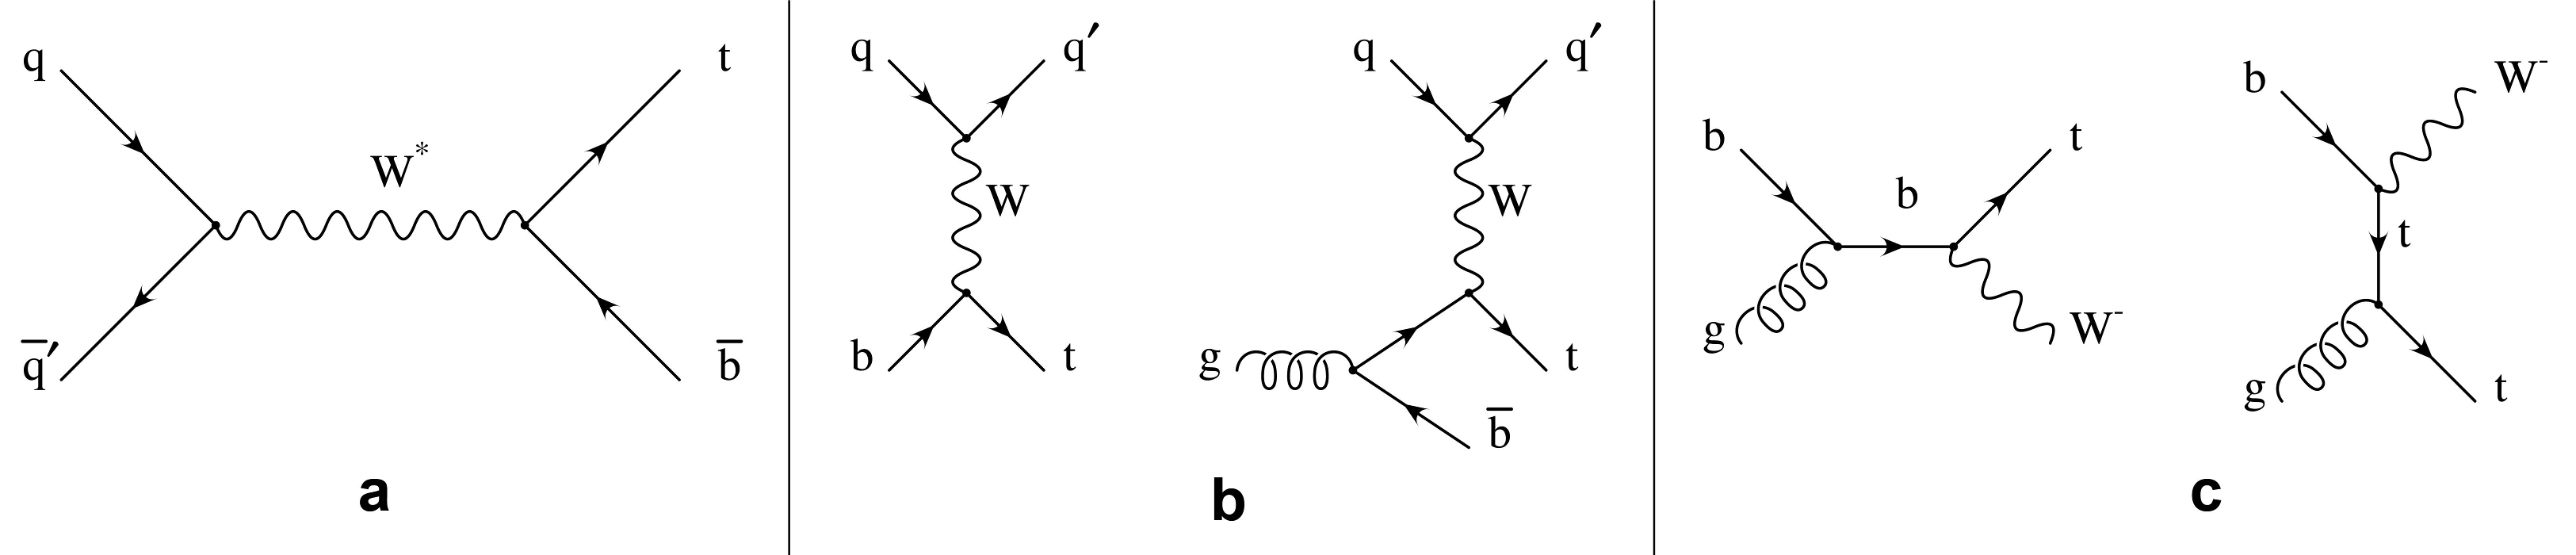
\includegraphics[width=1.\textwidth]{img/singletop}
    \caption[Produktionskanäle für ein einzelnes Top-Quark in Proton-Proton
        Kollisionen]
        {Produktion eines einzelnen Top-Quarks in Proton-Proton Kollisionen im
        s-Kanal (a), t-Kanal(b) und mit einem W-Boson im Ausgangszustand (c).}
    \label{fig:singletop}
\end{figure}

Für die Produktion im t-Kanal (b) wurde für die Simulation des Streuprozesses
\textsc{AcerMC} (\cite{Kersevan:2004yg}) als Generator verwendet, der eine
Schnittstelle zu \textsc{Pythia6} (\cite{1126-6708-2006-05-026}) zur
Beschreibung von Bremsstrahlung und Hadronisierung bereitstellt. Die beiden
anderen Kanäle (a) und (c) und die Produktion eines Top-Antitop Paares wurden
hingegen mit \textsc{MC@NLO} (\cite{Frixione:2002ik}) simuliert, einem
Generator, der auf nächsführender Ordnung \ac{QCD} Prozesse zu simulieren in
der Lage ist. Für die Top-Antitop Paarproduktion konnte von der oben bereits
erwähnten \textit{ZPrime} Gruppe der Wirkungsquerschnitt auf NNLO bestimmt
werden, was bei der weiter unten beschriebenen Skalierung der Monte-Carlos
relevant wird.

\subsubsection{Diboson}
Weitere Beiträge zur Untergrundabschätzung liefert die Simulation von der
Produktion zweier schwerer Eichbosonen. Dabei werden für jede Kombination, also
WW/WZ/ZZ separate Monte-Carlos generiert. Der hierfür verwendete Generator ist
\textsc{Herwig++} (\cite{Bahr:2008pv}), der in führender Ordnung die
Streuprozesse und Hadronisierung simuliert. Auch für diese Simulationen konnten
von der \textit{ZPrime} Gruppe die Wirkungsquerschnitte auf NLO bestimmt
werden.



\subsection{Skalierung}
Die generierten Monte-Carlo Simulationen entsprechen mit ihren
unterschiedlichen Wirkungsquerschnitten und der Zahl generierter Ereignisse
verschiedenen integrierten Luminositäten, weshalb zum Vergleich mit realen
Daten eine Skalierung notwendig wird. Man normiert dabei alle aus Monte-Carlos
erstellten Histogramme auf die äquivalente Luminosität in den Daten, mit einem
Skalierungsfaktor $s$:

\begin{equation}
    s = \frac{\sigma\cdot\epsilon\cdot L}{\sum_i^N w_{\text{pu},i}\cdot
    w_{\text{gen},i}}
    \label{eq:mc_scaling}
\end{equation}

Dabei bezeichnet $\sigma$ den Wirkungsquerschnitt des generierten Monte-Carlos
und $L$ die integrierte Luminosität des Datensatzes, auf den skaliert wird,
also im vorliegenden Fall $20.3 \fb^{-1}$. Anstelle durch die Gesamtzahl der
generierten Ereignisse zu dividieren, müssen die nicht-unitären Gewichte, wie
Pile-Up- und Generator-Ereignisgewicht, berücksichtigt werden und anstelle
durch deren Produkt, summiert über alle Ereignisse geteilt werden. Auf einige
der erzeugten Monte-Carlos wurde ein zusätzlicher Filter eingesetzt, um nicht
relevante Ereignisse\footnote{zum Beispiel Ereignisse deren Produktteilchen
nicht im angestrebten Phasenraum zu finden sind} zu unterdrücken. Die Effizienz
dieser Filter wird mit $\epsilon$ berücksichtigt.

Alle Ereigniszahlen, Wirkungsquerschnitte und Effizienzen sind in Anhang
\ref{appendix:monte_carlo_samples} in den jeweiligen Tabellen zu den
Monte-Carlo Simulationen zu finden.



%______________________________________________________________________________
%                                                                     Selektion 
\section{Selektion}
\label{data_sim_selection:selection}

\begin{itemize}
    \item \sout{Motivation für Schnitte (Untergrund-Diskriminierung)}
    \item Event-basierte Schnitte (Trigger, Detektor, primVertex)
    \item Elektron-basierte Schnitte (CC/CF, pT, ID, Autor, IQ)
    \item kurze erwähnung andere schnitte (MET,Jets,...)
\end{itemize}

Als \textit{Selektion} bezeichnet man die Gesamtheit von Kriterien, deren
Anwendung auf die vollständige Ereignismenge eines Datensatzes zu jener
Teilmenge von Ereignissen führt, die nur noch für die angestrebte Analyse
relevante Informationen enthält. Dies dient der Unterdrückung von
Untergrundbeiträgen und der gleichzeitigen Anreicherung mit Signalereignissen.
Als Kriterien kommen vielfältige Bedingungen an die enthaltenen Teilchen oder
das Ereignis an sich in Frage. Die einfachste und zugleich meist genutze Form
solcher Bedingungen sind simple Schnitte, bei denen einer Observablen ein
fester Grenzwert zugewiesen wird, sodann ein Über- oder Unterschreiten dieses
Wertes das Verwerfen des Ereignisses bedingt. Auch komplexere Forderungen sind
denkbar, wie beispielsweise die logische Verkettung von Ja/Nein-Entscheidungen
(siehe Trigger-Entscheidungen, Abschnitt \ref{}),
oder mehrdimensionale Schnittwerte auf der Basis multivariater Studien (siehe
Vorwärts-Elektron Identifikation, Abschnitt \ref{}).

Man unterscheidet dabei grob in Ereigbnis basierten Kriterien und solchen, die
Bedingungen an einzelne Teilchen stellen.

\subsection{Ereignisbasierte Selektionkriterien}






